\documentclass[10pt, 
               aspectratio=169,
               headline=default]{beamer} %[handout]

%% THEME               
\usetheme[block=fill]{metropolis}

%%% COLOR DEFINITIONS
\definecolor{mybackground}{RGB}{250, 247, 245}
\definecolor{color_primary}{RGB}{106, 141, 115}
\definecolor{color_secondary}{RGB}{244, 253, 217}
\definecolor{color_tertiary}{RGB}{228, 255, 225}
\definecolor{color_quaternary}{RGB}{240, 168, 104}

\definecolor{toc}{RGB}{255, 232, 194}
\definecolor{alerted}{RGB}{255, 232, 194}
\definecolor{tlike}{RGB}{255, 232, 194}
\definecolor{ftitle}{RGB}{255, 232, 194}

%% SET COLORS TO TEMPLATE
\setbeamercolor{background canvas}{bg=mybackground}
\setbeamercolor*{structure}{bg=color_secondary,fg=color_primary}

% \setbeamercolor*{palette primary}{use=structure,fg=white,bg=structure.fg}
% \setbeamercolor*{palette secondary}{use=structure,fg=white,bg=structure.fg!75}
% \setbeamercolor*{palette tertiary}{use=structure,fg=white,bg=structure.fg!50!black}
% \setbeamercolor*{palette quaternary}{fg=white,bg=black}

% \setbeamercolor{section in toc}{fg=black,bg=white}
% \setbeamercolor{alerted text}{use=structure,fg=structure.fg!50!black!80!black}

% \setbeamercolor{titlelike}{parent=palette primary,fg=structure.fg!50!black}
% \setbeamercolor{frametitle}{bg=gray!10!white,fg=color_secondary}

% \setbeamercolor*{titlelike}{parent=palette primary}
% \usepackage{beamerthemeshadow}
% \usecolortheme[named=SeaGreen]{structure}

%% MATH, FONTS, LAYOUT PACKAGES
\usepackage[utf8]{inputenc}
\usepackage{hyperref}
\usepackage{amsmath}
\usepackage{amssymb}
\usepackage{amsthm}
\usepackage{mathtools}
\usepackage{mwe}
\usepackage{listings}
\usepackage{multicol}
\usepackage{beton}
% \usepackage{fontspec}
\usepackage{xcolor}
\usepackage{verbatim}
\usepackage{caption}
\usepackage{subcaption}
\usepackage[backend=biber, doi=false, url=false]{biblatex}
\addbibresource{./BEC.bib}
\usepackage{csquotes}
\usepackage[makeroom]{cancel}
\usepackage{fancybox, graphicx}
\graphicspath{{figures}}
\usepackage{changepage}
%\usepackage{animate}
\usepackage{media9}
\usepackage{float}
\pagenumbering{roman}

%% 

\setlength{\marginparwidth}{1.5cm}




\makeatletter
\setbeamertemplate{headline}{%
  \vskip10pt % Increase the title bar height by adding 10pt vertical space
  \leavevmode

    \begin{beamercolorbox}[wd=\paperwidth,ht=1.2ex,dp=0.6ex]{frametitle}
        \hspace*{1ex}\insertframetitle%
    \end{beamercolorbox}%

}
\makeatother

% % Headline

%% footline numbering
\setbeamertemplate{footline}{\vspace*{1mm}\hfill
	\insertframenumber/\inserttotalframenumber\hfill\vspace*{1mm}}


\newcommand\nofoot[1]{%
  \begingroup
  \renewcommand\thefootnote{}\footnote{#1}%
  \addtocounter{footnote}{-1}%
  \endgroup
}


\makeatletter
\let\beamer@writeslidentry@miniframeson=\beamer@writeslidentry
\def\beamer@writeslidentry@miniframesoff{%
  \expandafter\beamer@ifempty\expandafter{\beamer@framestartpage}{}% does not happen normally
  {%else
    % removed \addtocontents commands
    \clearpage\beamer@notesactions%
  }
}
\newcommand*{\miniframeson}{\let\beamer@writeslidentry=\beamer@writeslidentry@miniframeson}
\newcommand*{\miniframesoff}{\let\beamer@writeslidentry=\beamer@writeslidentry@miniframesoff}
\makeatother

\title{Title}
\date{}


\titlegraphic{ \vspace{5cm}  \begin{minipage}{3cm}
  Francesco Lorenzi, \\ Luca Salasnich \\   
  \vspace{0.2cm} 
  \footnotesize{Where, when} 
\end{minipage}%
\hspace{0.5cm}
\begin{minipage}{5cm}
  
\includegraphics[width=1\textwidth]{logo/DFA.png}%
\end{minipage}
\hspace{1cm}
\begin{minipage}{4cm}
  
\includegraphics[width=1\textwidth]{logo/unipd-text.png}%
\end{minipage}%
  }

% \usefonttheme{structuresmallcapsserif}
\usepackage{textpos}

\usefonttheme{professionalfonts} % using non standard fonts for beamer
\usefonttheme{serif} % default family is serif

% remove navigation symbols from beamer theme
\beamertemplatenavigationsymbolsempty
\setbeamertemplate{footline}[frame number]
\setbeamertemplate{caption}{\raggedright\insertcaption\par}

\setbeamertemplate{headline}{%
    % \vspace{20pt}
    % \nointerlineskip%
    % \begin{beamercolorbox}[wd=\paperwidth,ht=1.2ex,dp=1.2ex]{frametitle}
    %     \hspace*{1ex}\insertframetitle%
    % \end{beamercolorbox}%
}

% \addtobeamertemplate{frametitle}{}{%
% \begin{textblock*}{100mm}(.85\textwidth,-2.1cm)
% \hspace{1cm}
\includegraphics[width = 0.2cm]{logo/DFA.png}%
% \end{textblock*}}

\begin{document}

\begin{frame}
    \maketitle
\end{frame}

%%%%%%%%%%%%%%%%%%%%%%%%%%%
% PRESENTATION OF MYSELF
%%%%%%%%%%%%%%%%%%%%%%%%%%%
\section{First topic}

\begin{frame}{Slide title}
I'm a student of ICT engineering and Photonics, with strong interest in fundamental topics in physical sciences and mathematical methods.\pause

\vspace{20pt}

\begin{columns}
	\begin{column}{.45\textwidth}
		\textbf{{\color{color_quaternary}Contribution of the Ph.D. program to my life}}
		\begin{itemize}
			\item Collaborate with highly-driven people in the field of physics of matter, and exchange deep scientific ideas.
			\item Expose myself to different fields of physics and learn far-reaching methodology.
		\end{itemize}
	\end{column}\pause

	\begin{column}{.45\textwidth}
		
		\textbf{{\color{color_quaternary}My contribution to the Ph.D. program}}
		\begin{itemize}
			\item Synthesize original ideas in physics of matter using concepts from my multidisciplinary background.
			\item Help building bridges between adjacent fields of physics, and engineering.
		\end{itemize}
        % \begin{figure}[l]
        %     \begin{subfigure}[b]{\textwidth}
        %          \includegraphics[width=0.8\textwidth]{images/bll2_quadrata.jpg}
        %     \end{subfigure}
        %     \vspace{20pt}
            
        %     \begin{subfigure}[b]{\textwidth}
        %         \includegraphics[width=0.8\textwidth]{images/me2_2.jpg}
        %     \end{subfigure}
        % \end{figure}
    \end{column}
\end{columns}
\end{frame}


%%%%%%%%%%%%%%%%%%%%%%%%%%%
%% RESEARCH PROJECT
%%%%%%%%%%%%%%%%%%%%%%%%%%%

\section{State of the art}

\begin{frame}{Frame with images and citations}
	\nofoot{\fullcite{khaykovich2002formation}}
	\vspace{-20pt}
	\begin{figure}
			\begin{subfigure}{0.55\textwidth}
				\centering
				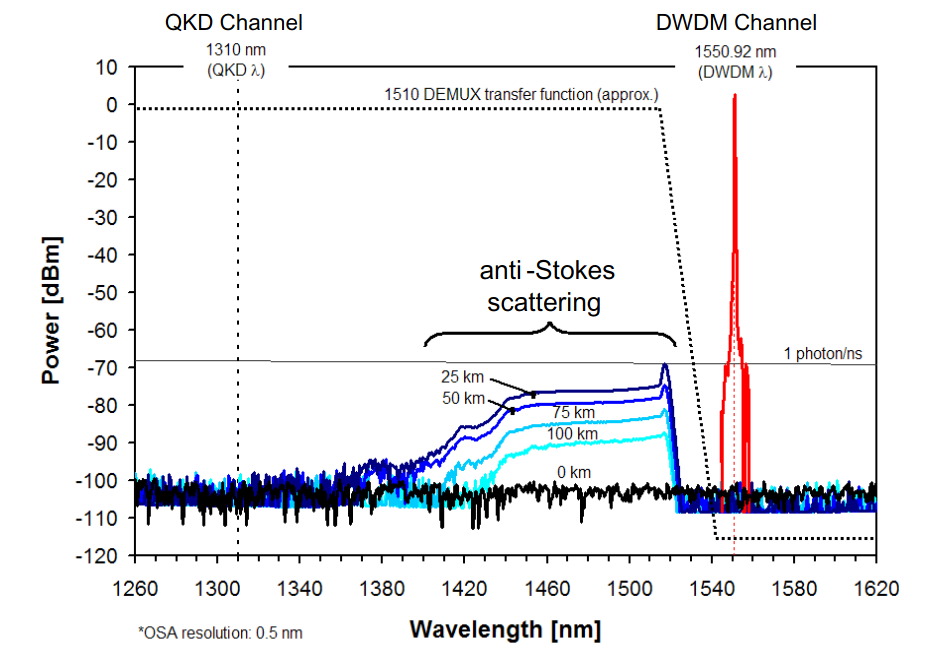
\includegraphics[width=\textwidth]{example.png}
			\end{subfigure}
			\hspace{10pt}
			\begin{subfigure}{0.40\textwidth}
				\centering
				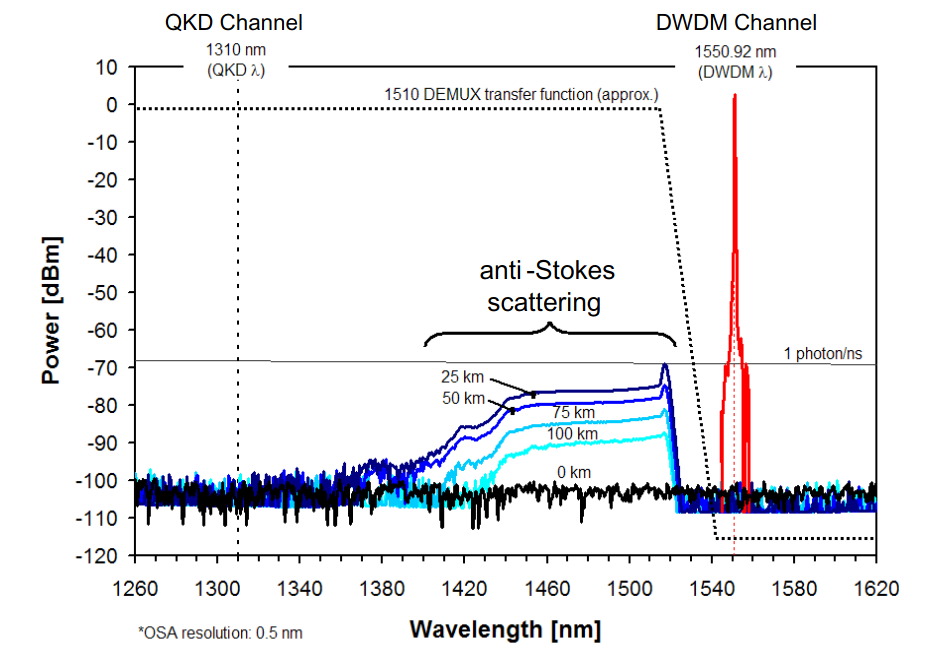
\includegraphics[width=\textwidth]{example.png}
				\caption{Transverse width for different interaction strengths}
				\vspace{30pt}
			\end{subfigure}
	\end{figure}
\begin{adjustwidth}{1cm}{1cm}
	\textit{Solitons} have been observed in $^7$Li BEC \cite{khaykovich2002formation}.\\
	They are "solitary waves", i.e. non-dispersive matter-waves which preserve the shape in time.\\
	They can be predicted from mean-field Gross-Pitaevskii equation.
	\end{adjustwidth}
\end{frame}

\begin{frame}{Frame with citation box}
\centering

\begin{minipage}{10cm}


    \begin{alertblock}{}
        ``The survey of the currently available results clearly demonstrates that there
        remains a \textit{vast room} for \textit{further theoretical} and experimental \textit{studies} of solitons and
        related self-trapped modes in photonics, \textit{BEC}, and other quickly developing areas of
        physics."
    \end{alertblock}
\end{minipage}

\begin{minipage}{11cm}
	\centering
	\vspace{20pt}
	The research activity starts from these premises!
	\vspace{20pt}
\end{minipage}
\nofoot{quote from Boris A Malomed and Dumitru Mihalache (2019) \cite{malomed2019nonlinear}.}
\end{frame}

\begin{frame}
	\centering
	\Huge{Thanks for the attention!}
\end{frame}

\begin{frame}[allowframebreaks]{Relevant references}
    %\nocite{*}
	\printbibliography
\end{frame}

\section*{Additional material}

\end{document}
